%!TEX root = ../thesis.tex
\chapter{The one with data and BOW\label{ch:dataandBOW}}

The main source of data for analysis is draw from the Twitter accounts of news-media organisations. In the 1950s, the widespread popularity of household television allowed TV broadcasting to become the primary tool for influencing public opinion in developed nations~\cite{diggs-brown_strategic_2011}.  This was a shift from a population that \emph{listened} to radio news, to a population that \emph{watched} news. 

The even more rapid rise of mobile internet and social media sites in the last two decades has caused another shift. No longer just a population that watch news at fixed time, or read regularly scheduled newspapers; the conveniences of the modern developed world allow individuals to consume news anytime, anywhere. As of 2019, 55\% of US adults get their news from social media either `often' or `sometimes'~ and 88\% state that `social media companies have at least some control over the mix of news people see'~'\cite{shearer_americans_2019}.

Given the importance of a free press and the role of social media sites in the delivery of news, this work aims to study the news on social media. To begin this task, we first define some common terms for clarity.

\begin{definition}[Social media]
	The platforms used to consume information by individuals in the public. E.g. Twitter, Facebook, Reddit.
\end{definition}

\begin{definition}[News-media]
	The organisations that are producing information about a broad range of current events and sharing that information with the public.
\end{definition}

\begin{definition}[News]
	The \emph{content} produced by news-media organisations. 
\end{definition}


\begin{definition}[Consumers]
	Individuals in the public that willingly seek out and consume news from news-media organisations.
\end{definition}

\section{Data}

% <allsides disscussion>
Using the media analysis source AllSides\footnote{www.allsides.com}, a collection of news-media organisations was found. The purpose of AllSides is to provide an open  analysis of political leanings of news sources~\cite{gable_media_2019}, and to aggregate news allowing consumers to view articles from different sides of the political spectrum. Each news source is labelled into one of 5 categories, {\color{Left}Left},
{\color{LeanLeft}Lean Left},
{\color{Center}Center},
{\color{LeanRight}Lean Right}, or
{\color{Right}Right}.
Any news source the ratings are determined internally using `blind surveys of people across the political spectrum, multi-partisan analysis, editorial reviews, third party data, and tens of thousands of user feedback ratings'~\cite{gable_media_2019}. News sources are only assigned to a single category, but do have an attached confidence rating that is provided from users selecting if they agree or disagree with the rating. An example of the ratings can be seen in \autoref{fig:allsidesmediabiaschart}.

\begin{figure}
	\centering
	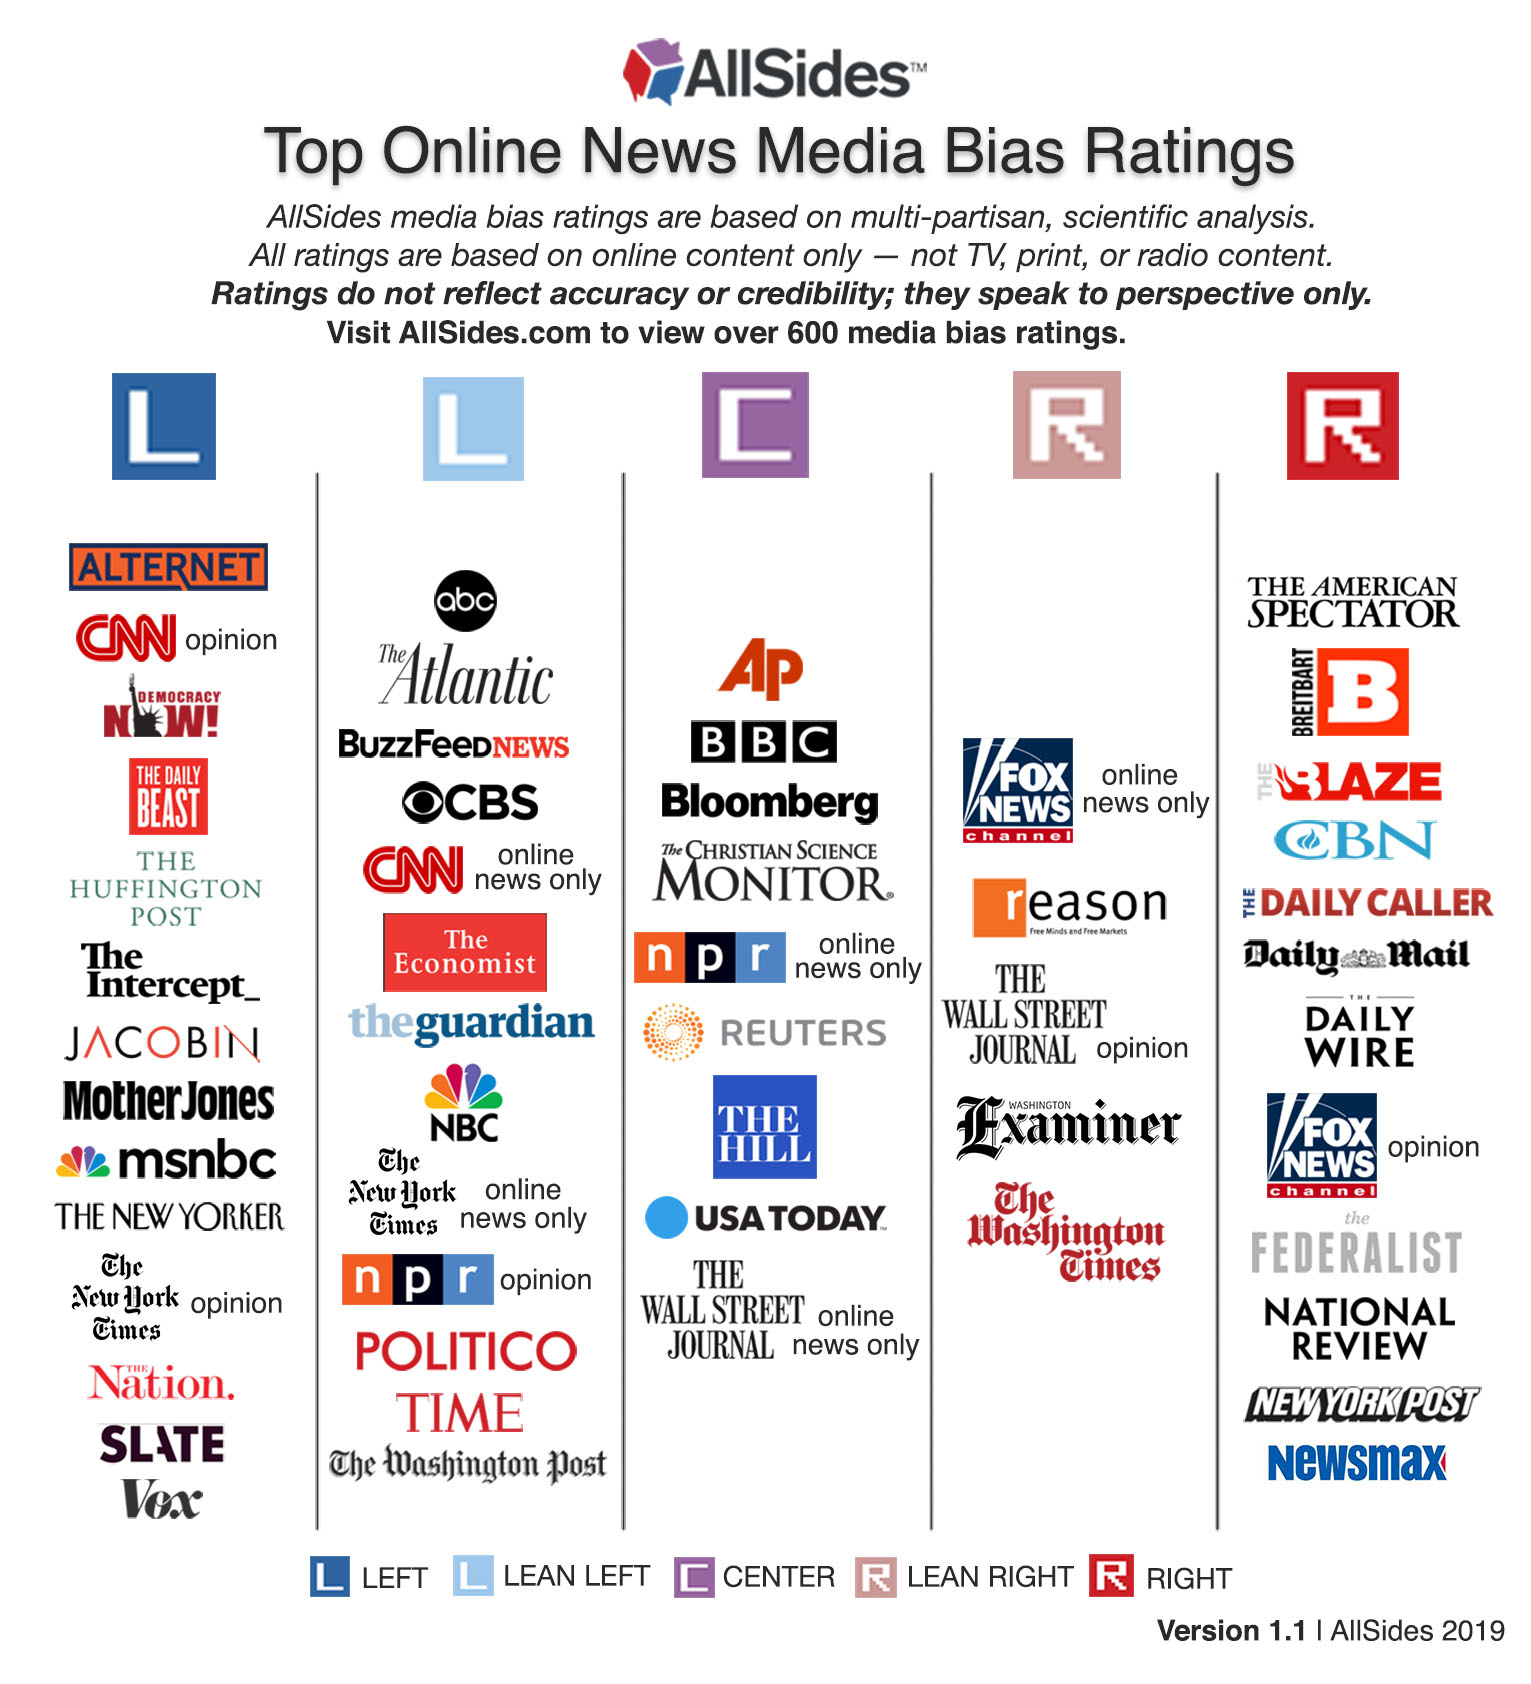
\includegraphics[width=0.9\linewidth]{chapter1/figs/AllSidesMediaBiasChart}
	\caption{An example collection of News-Media sites that have been classified into biases; sourced from Allsides website~\cite{gable_media_2019}}
	\label{fig:allsidesmediabiaschart}
\end{figure}
% </allsides disscussion>



% <sorting organisations>
From the website, a list of possible news sources was collected on February 1st, 2019. In this collection was organisation names, political bias', the number of user feedback ratings of the political bias, and, if available, the twitter handles associated with those sources. These collected news sources were broad, containing not just news-media organisations but authors, pundits and think tanks. 

To select an appropriate set of news-media organisation an examination and filtering process was undertaken. A source was only considered if it was a organisation (not an individual), that produced news content of a diverse range of topics. Many news sources were connected to think tanks or opinion groups, and only created news of a single topic or campaign. Further, if an news-media organisation has no twitter account or had less than 10,000 followers (a low bar in the social media world), then it was removed from the pool. This mainly removed inactive organisations and news organisation from small rural towns. Finally, a single source was removed as it was not in English, and a single source was removed as it was the smaller sister site that had all content as a subset of it's larger site.  The result of this filtering process is 170 news-media organisations and associated twitter accounts and categorised political bias'.  A list of all news-media organisations under analysis can be seen in \cite{app:accounts} and all removed sources and the removal justification can be seen in \autoref{appendix:tab:removed_accounts_0}.
% </sorting organisations>


%  <twitter collection>
Using the Twitter user handles associated with each of the news-media organisations, the history of all tweets for each account was collected using the Twitter application programming interface (API)\footnote{https://developer.twitter.com/en/docs} and web-scraping tools~\tocite{twint}. Of interest in this work are the tweets each news organisation tweeted between January 1st, 2019 to January 1st, 2020. 

Each major news-media organisation will tweet pieces of news multiple times throughout the day. The manner in which each organisation does this can differ and no standard format is used. The tweets often come in the form of single line description of articles, alongside a link to an article on the news-media organisation's website. The primary purpose of using social media sites to post these stories is to drive traffic to the organisation's website, wherein they can earn revenue from ad impressions. As such, the format of such news tweets is to extract core concepts from articles and frame them in their most essential and appealing way; in essence, they are trying to create so-called `click-bait' \tocite{something tot do with clickbait}. This format is desirable for our work as we want to explore how the language we use in news to appeal to consumers differs between organisations. This simplified format presents a reduced essence of this notion.

% breaking news
Twitter also serves another purpose for news-media organisations as a tool for breaking news. The modern 24 hour news cycle has had many effects on journalism, but chief among them is the need to produce breaking news at a lightning fast pace. The use of social media as a near instant tool for global public communication means that often no time can be wasted in publishing knowledge of a story, often while it is unfolding. Indeed, research has explored the role of Twitter for breaking news in the cases of the 2011 UK summer riots~\cite{vis_twitter_2013}, through activity providing real time updates over the four days, and in the case of the death of Osama Bin Laden in 2011~\cite{hu_breaking_2012}, where the news was leaked and spread virally through social media before any news-media organisations could fully verify and publish stories on the claim. These breaking news stories are sometimes, but not always, precedes by expressions such as ``\emph{Breaking News:}''. The inconsistent use of such a preamble can present challenge in our analysis of language moving forward, an \todo{will be explored more in this section}.
%  </twitter collection>

% <removal of inactive twitter accounts>
Using this collection method a total of 3,221,769 tweets were collected from the 170 news-media organisation official Twitter accounts in the 2019 calendar year. This represents an average number of tweets per day of above 50 tweets for each news organisation. In total, this appears a large useful corpus on text data for analysis. However, the activity level and consistency of output variety greatly between organisations. As can be seen in \autoref{fig:data_cleaning_average_tweet_activity}, some news organisations produce very little content on average. This can be explained through two mechanisms.

\begin{figure}
	\centering
	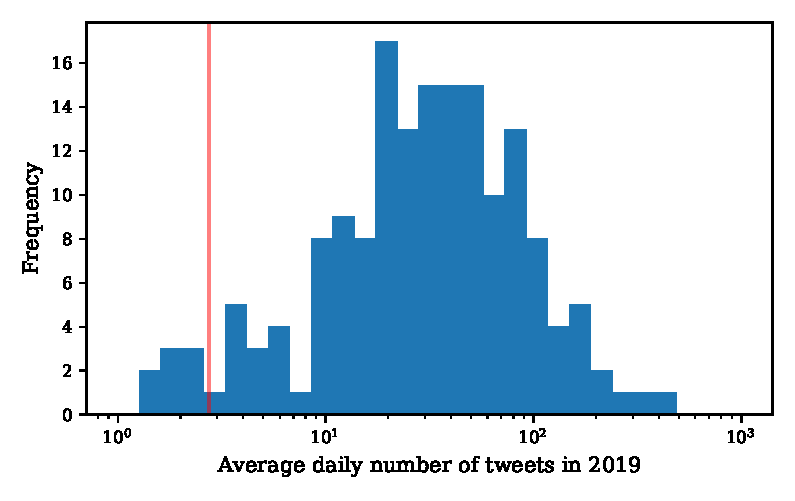
\includegraphics[width=0.7\linewidth]{chapter1/figs/averagetweetactivity}
	\caption{The average number of tweets produced each day during the 2019 calendar year for all 171 news-media organisations. The red line is the chosen threshold of 1000 tweets in the year, an average of 2.74 tweets per day.}
	\label{fig:data_cleaning_average_tweet_activity}
\end{figure}

Firstly, some organisations are not very active on social media. In particular, smaller organisations, which are typically less well resourced, place a lower priority on social media posting. This lowered tweet volume, presents a challenge for this work. In particular the use of bag of words tools and the non-parametric entropy estimator in \autoref{ch:crossentropy} require a substantial amount of text to reach meaningful results. As such, organisations that produced less that 1000 tweets in 2019 were removed from further consideration. This removed a total of 11 news-media organisations, listed in  \autoref{tab:data_removed_low_tweet_counts}.


\begin{table} 
	\centering
	\begin{tabular}{llr}
		\toprule
		News-media Organisation &    Bias  &  Number of tweets in 2019\\
		\midrule
		RealClearPolitics &      Center &  532 \\
		IJR  &  Lean Right &  777 \\
		WND News &         Right &  709 \\
		PRI &                Center &  346 \\
		EurekAlert! &            Center &  610 \\
		FAIR &     Center &  697 \\
		Crowdpac &            Center &  521 \\
		Inside Philanthropy &        Center &  781 \\
		Diplomatic Courier &         Center &  750 \\
		Peacock Panache &          Left &  198 \\
		Independent Voter &            Center &  303 \\
		\bottomrule
	\end{tabular}
\caption{Table of news-media organisations that were removed from data due to a low number of tweets in the 2019 calendar year.}
\label{tab:data_removed_low_tweet_counts}
\end{table}

Secondly, an issue was identified in long periods of inactivity of a few organisations. Five news-media organisations, for reasons unknown had large periods of time in which they did not post any tweets. These periods of time, spanning a few months, present key issues to our investigation. Moving forward we will consider time an important aspect of news, especially in the context of breaking news, as such these organisations are not only at a disadvantage in this space but present an anomaly in our data that hinders our ability to extract meaningful results from them. As such, these five organisations, listed in \autoref{tab:data_removed_inactive_period} were removed from further consideration and analysis.

\begin{table}
	\centering
	\begin{tabular}{ll}
		\toprule
		News-media Organisation &    Bias \\
		\midrule
		American Thinker  &      Right \\
		Pacific Standard &  Lean Left \\
		Philly.com  &  Lean Left \\
		Splinter &       Left \\
		ThinkProgress  &       Left \\
		\bottomrule
	\end{tabular}
	\caption{Table of news-media organisations that were removed from data due to long periods of inactivity.}
	\label{tab:data_removed_inactive_period}
\end{table}


To further confirm the validity of the sources in terms of their activity level over time, we examine the isolated daily activity of each news-media organisation. An activity curve for the New York Times can be seen in \autoref{fig:data_newyorktime_activity}. 
A clear weekly trend, wherein tweet activity is decreased, but not zero, during the weekends can bee seen in the New York Time activity, but is emblematic of a general trend seen in most news-media organisation. Further, many news-media organisations have distinct spikes that occur a key points during the year. These spikes indicate an extreme news day, wherein an organisation is covering a rapidly evolving breaking news story, or responding to major changes in discourse through the day. These are interesting and important features in the data, an worth keeping in mind during further analysis. The full collection of figures containing the daily activity levels of all included organisations can be seen in \autoref{app:activity}.

\begin{figure}
\centering
	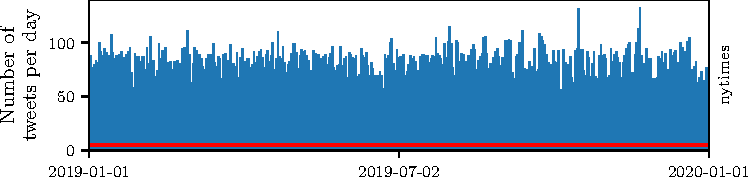
\includegraphics{appendix2/figs/tweet_times/nytimes.pdf}
	\caption{Twitter activity over 2019 for `The New York Times'.
		Twitter handle is `nytimes' with 44800317 followers and 31029 total tweets in 2019. A reference value of 5 tweets per day is shown in red. This is only one news-media organisation and all other activity figures for other organisations are available in \autoref{app:activity}}
	\label{fig:data_newyorktime_activity}
\end{figure}

With this now activity-level cleaned data, our news-media organisations have a slightly higher average number of tweets per day of 52.97. With the total number of remaining tweets at 2,977,980.
% </removal of inactive twitter accounts>


% <metadata>
As a result of this filtering we are left with 154 news-media organisations with complete data for the 2019 calendar year. Of these organisations the bias distribution is still somewhat representative of social media. \tocite{find a source that discusses why left wing is more popular on social media.} In total there are 73 organisations in the left half of the bias spectrum, 44 in the centre and 37 on the right; expanded on in \autoref{fig:data_number_of_bias_organisations}. This distribution, although shifted towards the left, still provides ample sources for the effect of bias to be explored further in this work, with keen attention to the potential impact of the skewed distribution. 

\begin{table}[h]
	\centering
	\begin{tabular}{lr}
		\toprule
		Bias &   Number of Organisations \\
		\midrule
		{\color{Left} Left }&  31 \\
		{\color{LeanLeft} Lean Left }&  42 \\
		{\color{Center} Center }&  44 \\
		{\color{LeanRight} Lean Right }&  16 \\
		{\color{Right} Right }&  21 \\
		\bottomrule
	\end{tabular}
	\caption{The number of news-media organisations in each political bias classification in our data.}
	\label{fig:data_number_of_bias_organisations}
\end{table}


From the news-media Twitter accounts we can also access metadata about the organisation. Two useful such pieces of metadata are the geographic location, and the number of followers on twitter.

% location data
On the Twiiter account of each news-media organisation they can elect to provide a text-based `location'. In some cases this option can be used for other purposes, such for self promotion (e.g. the \emph{New York Daily} states it's location as `\texttt{New York City  /  fb.com/nydailynews}') and many organisations have elected to leave the field blank. 
Of the organisation with locations, these can be difficult to disambiguate and compare. In situations were multiple cities or locations are defined, the largest possible inclusion was taken. For example `\texttt{New York and the World}' would become `Worldwide' in our classification, as would `\texttt{NYC, London, Paris, Hong Kong}'. These classifications were done manually due to the complexity of possible locations, and is summarised in  \autoref{tab:data_locations}.

\begin{table}
	\centering
	\begin{tabular}{lr}
		\toprule
		Location &  Counts \\
		\midrule
		New York &      34 \\
		Washington, D.C. &      20 \\
		Cafilforna &      11 \\
		Other US City &      44 \\
		General US &       8 \\
		Worldwide &       6 \\
		United Kingdom &       5 \\
		Qatar &       1 \\
		Pakistan &       1 \\
		Korea  &       1 \\
		Unspecified or Unclear &      43 \\
		\bottomrule
	\end{tabular}
	\caption{The aggregated self-defined locations of news-media organisation according to their Twitter account metadata. }
	\label{tab:data_locations}
\end{table}


% follower distributions
The number of followers a news-media organisation has on Twitter is an important metric, as it underpins the default mechanism through which people consume the news content produced. Although other algorithm news-feed  behaviours provide an important effect, the follower count plays a role in such a feed and is an effective metric of `success' in the eyes of the news-media organisations.

The most followed organisation in the data is \emph{The New York Times} with 44800317 accounts following at the time of collection in \todo{time of collection}. The least followed account included in the data is \todo{least followed account}. Interestingly, the follower counts are slightly higher for left biased organisations than for the right, in addition to be more numerous. This is shown via the followers distributions for each bias in \autoref{fig:data_number_of_follow_by_bias_raincloud}, which is indicative of the larger trend in social media of slightly left leaning demographics~\cite{mellon_twitter_2017}.

\begin{figure}
	\centering
	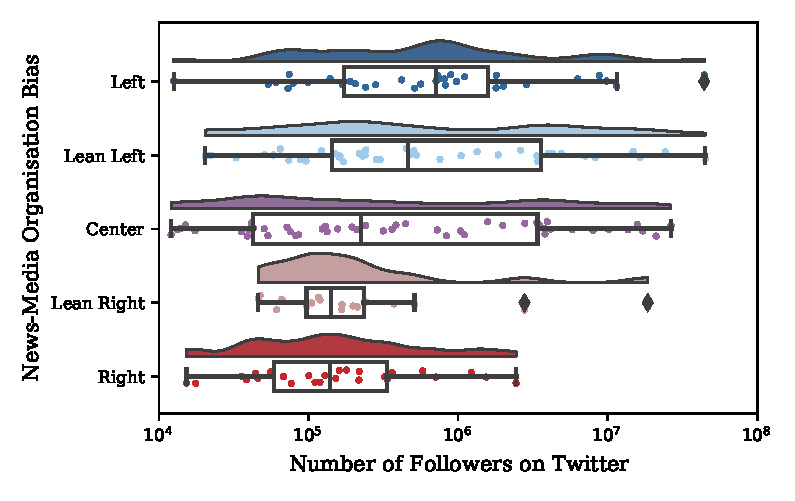
\includegraphics[width=\textwidth]{chapter1/figs/number_of_follow_by_bias_raincloud}
	\caption{Number of followers on Twitter of news-media organisations included in the data. Grouping is according to Allsides bias.}
	\label{fig:data_number_of_follow_by_bias_raincloud}
\end{figure}

% </metadata>

%\the\textwidth
%
%% somewhere maybe summary
%60054638 words
